\documentclass[]{article}
\usepackage{mathtools}
\usepackage[pdftex]{graphicx}	
\usepackage{amsmath,amsfonts,amsthm}	
\usepackage{tikz}

\usepackage{sidecap}
\usepackage{polski}
\usepackage[utf8]{inputenc}


\usetikzlibrary{chains, positioning}
\newtheorem{theorem}{Twierdzenie}[section]
\newtheorem{lemma}[theorem]{Lemma}
\newtheorem{proposition}[theorem]{Proposition}
\newtheorem{corollary}[theorem]{Corollary}

\theoremstyle{definition}
\newtheorem{definition}{Definicja}[section]

\usetikzlibrary{calc,arrows}

%opening
\title{Sieci neuronowe są uniwersalnymi aproksymatorami}
\author{Rafa\l \vspace{1cm} Skrzypiec}
\date{}
\begin{document}
\maketitle
Co jeszcze?
\begin{itemize}
	\item cytowania
	\item definicje i twierdzenia z polskiej literatury
	\item podpisy obrazków po polsku?
	
\end{itemize}
\begin{center}
	
	
	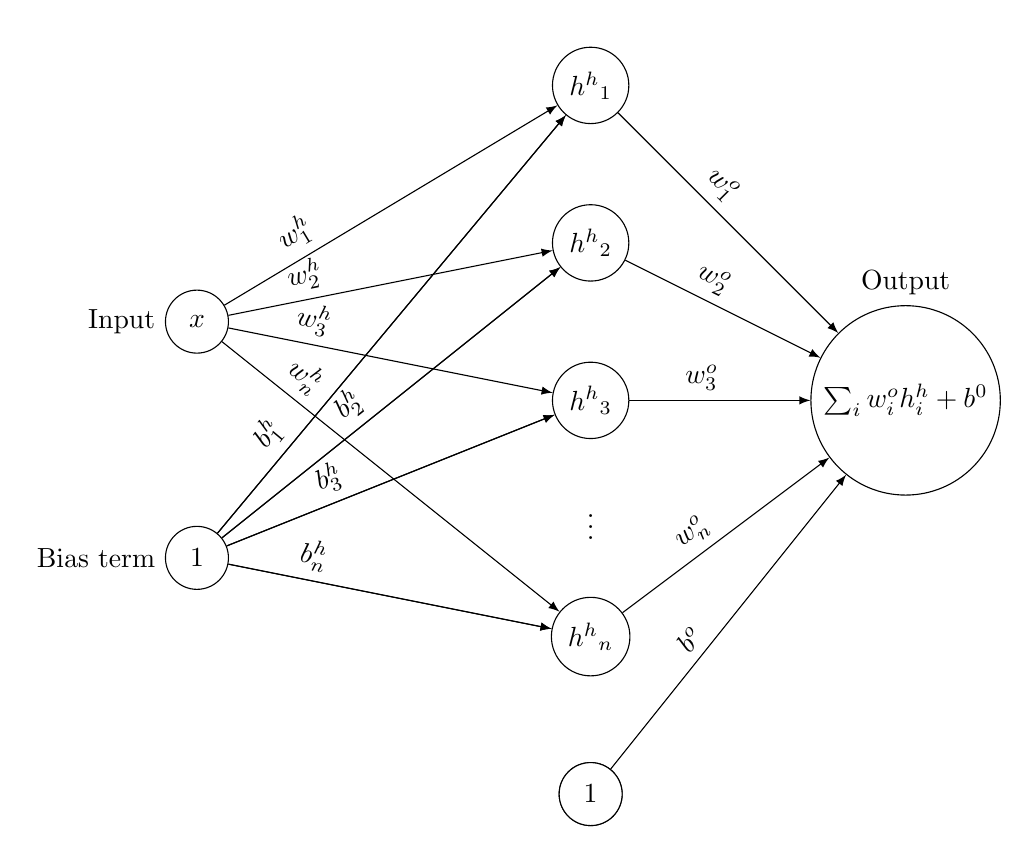
\begin{tikzpicture}
	[   cnode/.style={draw=black,draw=black,fill=#1,minimum width=8mm,circle},
	]
	\tikzset{normal arrow/.style={draw,-latex}}
	\node[cnode=white,label=90:Output] (s) at (9,-6) {$\sum_{i} w^o_{i} h^h_i + b^0$};
	\node[cnode=white,label=180:Bias term] (x-2) at (0,-8) {1};
	\node[cnode=white,label=180:] (p-5) at (5,-11) {1};
	\node at (5,-7.5) {$\vdots$};
	
	\node[cnode=white,label=180:Input] (x-1) at (0,-5) {$x$};
	
	\foreach \x in {1,...,5}
	{
		\pgfmathparse{\x<4 ? \x : "n"}	   
		\ifnum \x = 4
		
		
		\node[cnode=white,label=90:] (p-\x) at (5,{-2.*\x-div(\x,4)}) {${h^h}_n$};
		
		\else
		
		\ifnum \x = 5
		
		
		\node[cnode=white,label=90:] (p-\x) at (5,{-2*\x-div(\x,4)}) {$ 1 $};
		
		\else
		
		\node[cnode=white,label=90:] (p-\x) at (5,{-2*\x-div(\x,4)}) {${h^h}_{\x}$};
		
		\fi
		
		
		\fi
		\ifnum \x = 5
		\path[normal arrow] (p-\x) -- node[above,sloped,pos=0.4] {$b^{o}$} (s);
		\else
		\path[normal arrow] (p-\x) -- node[above,sloped,pos=0.4] {$w^o_{\pgfmathresult}$} (s);
		\fi
	}
	
	
	\foreach \x in {1,...,2}
	{   
		\foreach \y in {1,...,4}
		{   
			\ifnum \x=1
			\ifnum \y=4
			\path[normal arrow] (x-\x) -- (p-\y) node[above,sloped,pos=0.2] {$w^h_{n}$};
			
			\else
			\ifnum \y=5
			\path[normal arrow] (x-\x) -- (p-\y) node[below,sloped,pos=0.15] {$w_{w n+1}$};
			\else 
			\path[normal arrow] (x-\x) -- (p-\y) node[above,sloped,pos=0.25] {$w^h_{\y}$};
			
			\fi
			\fi
			\else
			\path[normal arrow] (x-\x) -- (p-\y); 		
			\fi
			
			\ifnum \x=2
				\ifnum \y=4
				\path[normal arrow] (x-\x) -- (p-\y) node[above,sloped,pos=0.25] {$b^h_{n}$};
					\else
				\ifnum \y=2
				\path[normal arrow] (x-\x) -- (p-\y) node[above,sloped,pos=0.42] {$b^h_{\y}$};
					\else
				\ifnum \y=3
								\path[normal arrow] (x-\x) -- (p-\y) node[above,sloped,pos=0.34] {$b^h_{\y}$};
				
				\else
				
					\path[normal arrow] (x-\x) -- (p-\y) node[above,sloped,pos=0.2] {$b^h_{\y}$};
					\fi
					\fi
				\fi
			\fi
			%\draw (x-\x) -- (p-\y) node[above,sloped,pos=0.3] {$\omega_{\x\y}$};
		}
	}
	\end{tikzpicture}
	
\end{center}


\newpage
\section{Uniwersalne twierdzenie aproksymacyjne}

Według uniwersalnego twierdzenia aproksymacyjnego jednokierunkowa sieć neuronowa z jedną warstwą ukrytą i skończoną ale wystarczająco dużą liczbą neuronów, może przybliżyć z dowolną dokładnością każdą funkcję.

W 1989 roku Cybenko [cytowanie] udowodnił uniwersalne twierdzenie aproksymacyjne dla jednokierunkowej sieci neuronowej z sigmoidalną funkcją aktywacji. Jeszcze w tym samym roku, po pracy Cybenki ukazała się praca Hornika, Stinchcombe'a and White'a, którzy udowodnili prawdziwość powyższego twierdzenia dla dowolnej funkcji aktywacji.

Funkcje sigmoidalne to rodzina funkcji szeroko stosowanych w jednokierunkowych sieciach neuronowych, szczególnie tych stworzonych do celów regresji. W tej części zaprezentuję dowód uniwersalnego twierdzenia aproksymacyjnego podany przez Cybenkę w 1989 roku, następnie zademonstruję dowód wizualny posługując się sigmoidą jako funkcją aktywacji.



\subsection{Przybliżenie przez kombinację liniową funkcji sigmoidalnych}

Niech $I_n$ oznacza $n$-wymiarową jednostkową kostkę , $[0,1]^n$. $C(I_n)$ to przestrzeń ciągłych funkjci na $I_n$. Dodatkowo, niech $M(I_n)$ oznacza przestrzeń skończonych, regularnych miar borelowskich na $n$-wymiarowej kostce jednostkowej $I_n$.

\begin{definition}
Miara $\mu$ jest regularna jeśli dla każdego mierzelnego zbioru $A$, $\mu(A)$ równa się supremum miar zamkniętych podzbiorów $A$ i infimum otwartych nadzbiorów $A$. [Probability measures on metric spaces K.R. Parthasarathy]	
\end{definition}
 
 
%\begin{definition} Zobaczymy czy się przyda
%	$f:I_n \rightarrow C(I_n),$
%	$||f|| = \sup {|f(x)| : x \in I_n }$.
%\end{definition}
% 
% 
% $||f||$ is used to denote the supremum norm of an $f \in C(I_n)$. 

\begin{definition}
	Funkcja $\sigma: \mathbb{R} \rightarrow \mathbb{R}$ jest funkcją sigmoidalną jeśli
	\begin{eqnarray*}
		\sigma(x) \rightarrow \begin{cases} 1 \;\;\;\text{as} &x \rightarrow +\infty\\ 0 \;\;\;\text{as} &x \rightarrow -\infty\end{cases}
	\end{eqnarray*}
	
\end{definition}



\begin{definition}
Funkcja $\sigma$ jest funkcją dyskryminaczyjną jeśli dla miary $\mu \in M(I_n)$ zachodzi 

\begin{equation}
\int_{I_n} \sigma \left( w^\mathsf{T}x + b_0 \right) d\mu(x) = 0
\end{equation}
dla każdego $w\in \mathbb{R}$ i $b_0 \in \mathbb{R}$ co implikuje, że $\mu = 0$.
	
\end{definition}


\begin{theorem}
Każda ograniczona, mierzalna funkcja sigmoidalna $\sigma$ jest funkcją dyskryminacyjną. W szczególności każda ciągła funkcja sigmoidalna jest dyskryminacyjna.
[cytowanie Cybenko]
\end{theorem}

Dowód uniwesalnego twierdzenia aproksymacyjnego przy wykorzystaniu funkcji sigmoidalnych wymaga wprowadzenia kilku przydatnych definicji i twierdzeń. Pierwsze z nich to twierdzenie Hahna-Banacha, które formułuje możliwość rozszerzenia każdego ograniczonego funkcjonału liniowego z podprzestrzeni unormowanej na całą podprzestrzeń, przy zachowaniu jego właściwości.


\begin{theorem}[Twierdzenie Hahna-Banacha]
	
	
	Niech $X$ to rzeczywista przestrzeń wektorowa, $p$ to funkcja rzeczywista zdefiniowana na $X$ spełniająca
	
	$$	p \left(\alpha x + (1-\alpha) y \right) \leq \alpha p(x)  + (1 - \alpha)p(y) \;\;\;\;\;\; \forall \alpha \in \left[0,1\right], x, y \in X$$
	
	
	Przypuśmy, że $\lambda$ to funkcjonał liniowy zdefiniowany na zbiorze $Y\subset X $, który spełnia
	$$\lambda(x) \leq p(x) \;\;\;\;\;\; \forall x \in Y.$$
	
	
	Wtedy istnieje funkcjonał liniowy $\Lambda$ zdefiniowany na $X$ spełniający
	$$\Lambda(x) \leq p(x) \;\;\;\;\;\; \forall x \in X,$$
	
	tak, że
	
	$$\Lambda(x) = \lambda(x) \;\;\;\;\;\; \forall x \in Y.$$
	

Reed \& Simon (1980), Methods of Modern Mathematical Physics. Functional Analysis
\end{theorem}


\begin{definition}	
	
	Przestrzeń $\mathcal{L}\left(\mathcal{H}, \mathbb{C}\right)$ nazywana jest przestrzenią dualną przestrzeni Hilberta $\mathcal{H}$ i oznaczamy ją przez $\mathcal{H^*}$. Elementy $\mathcal{H^*}$ nazywane są ciągłymi funkcjonałami liniowymi.
	
	
Reed \& Simon (1980), Methods of Modern Mathematical Physics. Functional Analysis
	
\end{definition}	


Twierdzenie Riesza opisuje przestrzeń $\mathcal{H^*}$.  

	
\begin{theorem}[Twierdzenie Riesza (znaleźć polskie źródło)]
	
Dla każdego $T \in \mathcal{H^*}$, istnieje unikalne $y_T \in \mathcal{H}$ takie, że $$T(x) = \langle y_T, x \rangle \;\;\;\;\;\; \forall x \in \mathcal{H} $$
	
	
Ponadto $$||y_T ||_{\mathcal{H}}  = ||T||_{\mathcal{H^*}}$$

Reed \& Simon (1980), Methods of Modern Mathematical Physics. Functional Analysis

\end{theorem}


\begin{theorem}[]
	
	Niech $\sigma$ będzie ciągłą funkcją dyskryminacyjną, wtedy skończona suma
	
\begin{equation}
G\left(x\right) = \sum_{i=1}^{N} w^{o}_i \sigma\left({w^h_i}^{\mathsf{T}}x + b^h_i\right)
\end{equation}

jest gęsta w $C(I_n)$. Innymi słowy, dla danej funkcji $f \in C(I_n)$ i $\epsilon >0$, istnieje suma

$G(x)$ mająca powyższą postać, dla której

$$
|G(x) - f(x)| < \epsilon \;\;\;\;\;\;\;\; \forall x \in I_n
$$
\end{theorem}

\begin{proof}


Niech $S \subset C(I_n)$ będzie zbiorem funkcji w postaci $G(x)$ lub w innych słowach - zbiorem sieci neuronowych. Z pewnością $S$ jest podprzestrzenią liniową $C(I_n)$. Jeśli $S$ jest gęsty, domknięcie $S$ jest całą przestrzenią $C(I_n)$.

Przyjmijmy, że domknięcie $S$ nie jest całą przestrzenią $C(I_n)$. Wtedy domknięcie $S$ -- $S'$ jest domkniętą podprzestrzenią $C(I_n)$. Przez twierdzenie Hahna-Banacha, istnieje ograniczony funkcjonał liniowy na $C(I_n)$, nazwijmy go $L$, z własnością, że $L \neq 0$ ale $L(S') = L(S) = 0$.

Przez twierdzenie Riesza, ograniczony funkcjonał liniowy $L$ ma postać

$$
L(h) = \int_{I_n} h(x)d\mu(x)
$$

dla $\mu \in M(I_n)$, dla każdego $h \in C(I_n)$. W szczególności, odkąd $\sigma(w^\mathsf{T}x + b)$  $\in S'$ dla każdego $w$ i $b$, musi zachodzić

$$
\int_{I_n} \sigma \left(w^\mathsf{T}x + b \right) d\mu(x) = 0 
$$

Jednakże, założyliśmy, że $\sigma$ jest funkcją dyskryminacyjną, ten warunek implikuje, że $\mu = 0$ co jest sprzeczne z naszym założeniem. Stąd, podprzestrzeń $S$ jest gęsta w $C(I_n)$.

Pokazuje to, że suma

$$
G\left(x\right) = \sum_{i=1}^{N} w^{o}_i \sigma\left({w^h_i}^{\mathsf{T}}x + b^h_i\right)
$$

jest gęsta w $C(I_n)$ pod warunkiem, że $\sigma$ jest ciągła i dyskryminacyjna.

Z twierdzenia wynika, że każda sieć neuronowa o wystarczająco dużej liczbie neuronów w jednej warstwie ukrytej i sigmoidalną funkcją aktywacyjną może z dowolną dokładnością przybliżyć przebieg każdej funkcji.

\end{proof}

\newpage

\section{Dowód wizualny}

\begin{figure}[h!]
	\centering
	\includegraphics[width=\linewidth]{cybenko14_12_1}

\end{figure}

\begin{figure}[h!]
	\centering
	\includegraphics[width=\linewidth]{mse}

\end{figure}




%\begin{table}
%		\begin{center}
%	\begin{tabular}{ | l | c | }
%		\hline
%		Number of hidden neurons & Mean squared error \\ \hline
%		1 & 0.00942516615858  \\ \hline
%		2 & 0.00277472585580  \\ \hline
%		3 & 0.00135999931016  \\ \hline
%		4 & 5.33546419190e-05  \\ \hline
%		10 & 1.70243920789e-06  \\ \hline
%		100 & 1.11243069317e-06  \\ \hline
%		\hline
%	\end{tabular}
%		\end{center}
%\end{table}



\newpage
\subsection{Dane}

Zbiór danych treningowych zawiera $m$ jednowymiarowych próbek zadanych przez wektory $X \in \mathbb{R}^{1\times m}$ i odpowiadające im wyniki $Y\in \mathbb{R}^{1\times m}$.



\subsection{Parametry}

Sieć ma dwie warstwy: 1) ukryta, zawierająca $L$ neuronów i 2) wyjściowa, składająca się z $1$ neuronu. Warstwy są zdefiniowane przez:

1. parametry wartstwy ukrytej, które odwzorowują $1$-wymiarowe wektory wejściowe w aktywacje $L$ neuronów:
macierz wag $W^h\in\mathbb{R}^{L\times 1	}$ i wektor parametru bias $b^h\in\mathbb{R}^{L\times 1}$,

2. parametry wartstwy wyjściowe, które odwzorowują $L$-wymiarowy wektor aktywacji neuronów ukrytych w jeden neuron wartstwy wyjściowej:
macierz wag $W^o\in{1\times L}$ i wektor bias $b^o\in\mathbb{R}^{1\times 1}$.


\subsection{Propagacja sygnału}

Wejście każdego neuronu w warstwie ukrytej jest iloczynem danych wejściowych i odpowiadającej im wagi plus parametr bias. Na przykład dla $i$-tego przykładu danych wejściowych, w $l$-tym neuronie mamy

\begin{equation}
{a^h}^{(i)}_l = {W^h}_{l}x^{(i)} + {b^h}_l
\end{equation}

%Wejście wszystkich neuronów dla wszystkich przykładów może być wyrażone przez macierze, używając mnożenia macierzy oraz broadcastingu (możliwości dodania wektora kolumnowego do wszystkich wektorów kolumnowych w macierzy) mamy

%\begin{equation}
%{a^h} = W^h\cdot x + b^h
%\end{equation}
%Co w Pythonie można zapisać jako $ah = W.dot(x) + b$


Funkcją aktywacyjną neuronów jest sigmoida $\sigma(a) = \frac{1}{1+e^{-a}}$, jako argument przyjmuje ona wejście neuronów:

\begin{equation}
{h^h}^{(i)}_l=\sigma({a^h}^{(i)}_l)
\end{equation}


Neuron warstwy wyjściowej zawiera sumę iloczynów aktywacji neuronów i odpowiadających im wag plus parametr bias. Dla $i$-tego przykładu mamy

\begin{equation}
\begin{split}
{a^o}^{(i)} &= \sum_{l} {W^o}_l{h^h}^{(i)}_l + {b^o} \\
& = \sum_{l} {W^o}_l\sigma({a^h}^{(i)}_l) + {b^o} \\
& = \sum_{l} {W^o}_l\sigma({W^h}_{l}x^{(i)} + {b^h}_l) + {b^o}
\end{split}
\end{equation}

Jako funkcja straty zostanie wykorzystany błąd średniokwadratowy

\begin{equation}
\begin{split}
J^{(i)}(\Theta) &= \frac{1}{2} \left( y^{(i)}- a^{o{(i)}}  \right)  ^2 \\
J(\Theta) &= \frac{1}{m}\sum_{i=1}^m J^{(i)}(\Theta)= \frac{1}{2m}\sum_{i=1}^m \left( y^{(i)}- a^{o{(i)}}  \right)  ^2  .
\end{split}
\end{equation}


\subsection{Propagacja wsteczna}


Użycie reguły łańcuchowej umożliwia obliczenie gradientu funkcji straty względem parametrów sieci neuronowej.

Na początku policzmy gradient względem wyniku wartstwy wyjściowej.



\begin{equation}
\frac{\partial J}{\partial {a^o}^{(i)}} = \frac{1}{m} \left( y^{(i)}- a^{o{(i)}}  \right),
\end{equation}

następnie policzmy gradient wyjścia neuronów ukrytych:

\begin{equation}
\frac{\partial J}{\partial {h^h}^{(i)}_l} = \frac{\partial J}{\partial {a^o}^{(i)}} \frac{\partial {a^o}^{(i)}}{\partial {h^h}^{(i)}_l} =  \frac{\partial J}{\partial {a^o}^{(i)}} {W^o}_{l},
\end{equation}

co umożliwia obliczenie gradientu względem wejścia neruonów ukrytych:

\begin{equation}
\frac{\partial J}{\partial {a^h}^{(i)}_l} = \frac{\partial J}{\partial {h^h}^{(i)}_l}\frac{\partial {h^h}^{(i)}_l}{\partial {a^h}^{(i)}_l} = \frac{\partial J}{\partial {h^h}^{(i)}_l} {h^h}^{(i)}_l(1-{h^h}^{(i)}_l) 
\end{equation}

gdzie została wykorzystana relacja
$$\frac{\partial \sigma(x)}{\partial x} = \sigma(x)(1-\sigma(x)).$$


Ostatecznie możemy policzyć gradienty względem parametrów sieci, np. dla warstwy wejściowej:

\begin{equation}
\frac{\partial J}{\partial {W^o}_{l}} = \sum_{i}\frac{\partial J}{\partial {a^o}^{(i)}}\frac{\partial {a^o}^{(i)}}{\partial {W^o}_{l}} = \sum_{i}\frac{\partial J}{\partial {a^o}^{(i)}}{h^h}^{(i)}_l,
\end{equation}

\begin{equation}
\frac{\partial J}{\partial {b^o}} = \sum_{i}\frac{\partial J}{\partial {a^o}^{(i)}}\frac{\partial {a^o}^{(i)}}{\partial {b^o}} = \sum_{i}\frac{\partial J}{\partial {a^o}^{(i)}}.
\end{equation}



\end{document}





wiki: "A sigmoid function is a mathematical function having a characteristic "S"-shaped curve or sigmoid curve. Often, sigmoid function refers to the special case of the logistic function defined by the formula"

$$
\sigma(x) = \frac{1}{1+e^{-x}}
$$





\begin{center}
	
	
	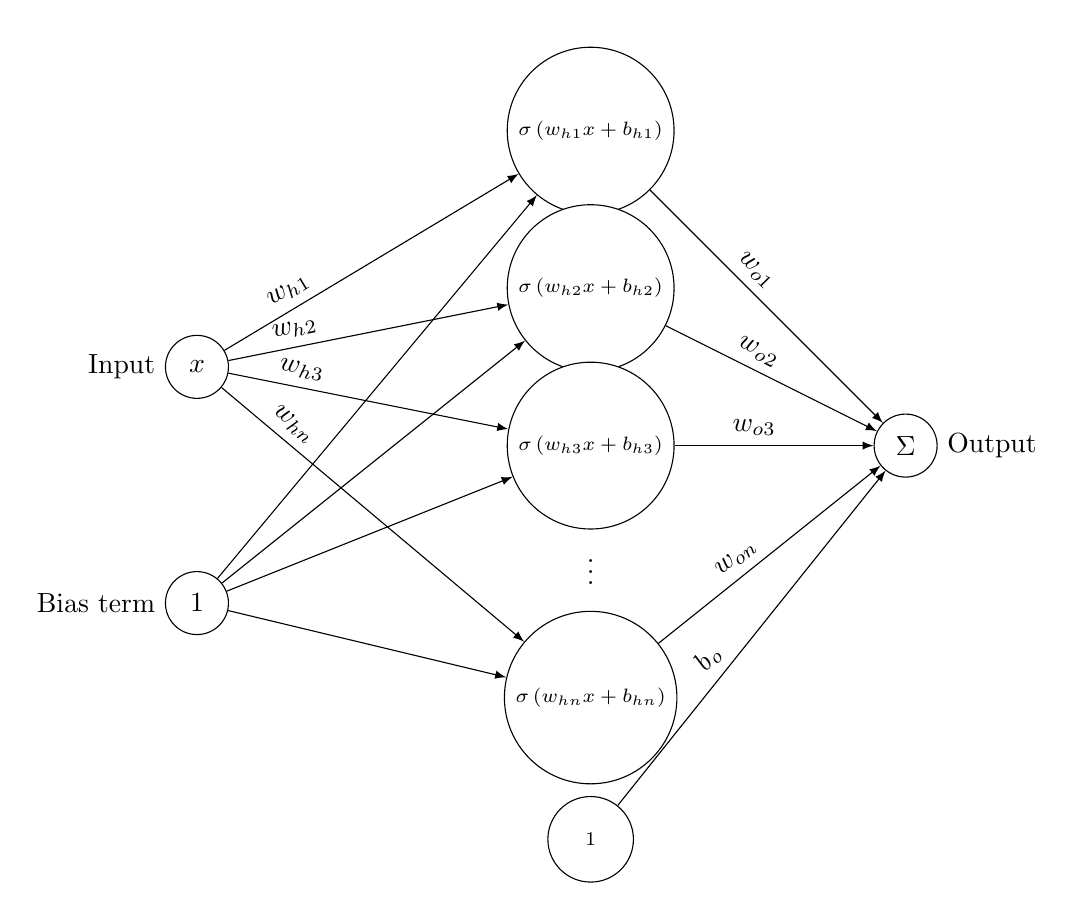
\begin{tikzpicture}
	[   cnode/.style={draw=black,draw=black,fill=#1,minimum width=8mm,circle},
	]
	\tikzset{normal arrow/.style={draw,-latex}}
	\node[cnode=white,label=0:Output] (s) at (9,-6) {$\Sigma$};
	\node[cnode=white,label=180:Bias term] (x-2) at (0,-8) {1};
	\node[cnode=white,label=180:] (p-5) at (5,-11) {1};
	\node at (5,-7.5) {$\vdots$};
	
	\node[cnode=white,label=180:Input] (x-1) at (0,-5) {$x$};
	
	\foreach \x in {1,...,5}
	{
		\pgfmathparse{\x<4 ? \x : "n"}	   
		\ifnum \x = 4
		
		
		\node[cnode=white,label=90:] (p-\x) at (5,{-2.05*\x-div(\x,4)}) {\scriptsize$\sigma\left(w_{hn}x + b_{hn}\right)$};
		
		\else
		
		\ifnum \x = 5
		
		
		\node[cnode=white,label=90:] (p-\x) at (5,{-2*\x-div(\x,4)}) {\scriptsize$\;\;\; \; 1 \; \;\;\;$};
		
		\else
		
		\node[cnode=white,label=90:] (p-\x) at (5,{-2*\x-div(\x,4)}) {\scriptsize$\sigma\left(w_{h\x}x + b_{h\x}\right)$};
		
		\fi
		
		
		\fi
		\ifnum \x = 5
		\path[normal arrow] (p-\x) -- node[above,sloped,pos=0.4] {$b_{o}$} (s);
		\else
		\path[normal arrow] (p-\x) -- node[above,sloped,pos=0.4] {$w_{o\pgfmathresult}$} (s);
		\fi
	}
	
	
	\foreach \x in {1,...,2}
	{   
		\foreach \y in {1,...,4}
		{   
			\ifnum \x=1
			\ifnum \y=4
			\path[normal arrow] (x-\x) -- (p-\y) node[above,sloped,pos=0.2] {$w_{h n}$};
			
			
			\else
			\ifnum \y=5
			\path[normal arrow] (x-\x) -- (p-\y) node[below,sloped,pos=0.15] {$w_{w n+1}$};
			\else 
			\path[normal arrow] (x-\x) -- (p-\y) node[above,sloped,pos=0.25] {$w_{h\y}$};
			
			\fi
			\fi
			\else
			\path[normal arrow] (x-\x) -- (p-\y); 
			
			\fi
			
			%\draw (x-\x) -- (p-\y) node[above,sloped,pos=0.3] {$\omega_{\x\y}$};
		}
	}
	\end{tikzpicture}
	
\end{center}



\def\layersep{2.5cm}
\begin{center}
	
	
	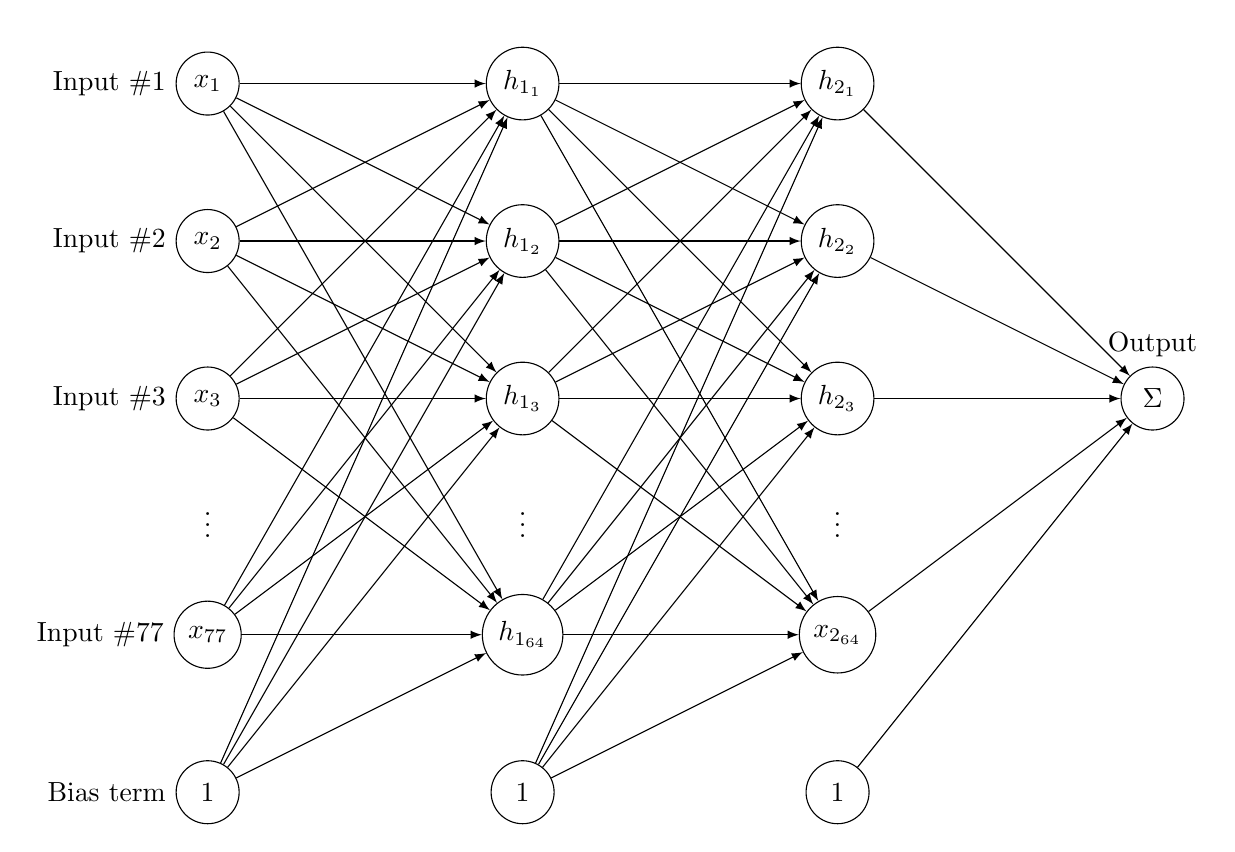
\begin{tikzpicture}
	[   cnode/.style={draw=black,draw=black,fill=#1,minimum width=8mm,circle},
	]
	\tikzset{normal arrow/.style={draw,-latex}}
	\node[cnode=white,label=90:Output] (s) at (12,-6) {$\Sigma$};
	\node at (0,-7.5) {$\vdots$};
	
	\node[cnode=white,label=180:Bias term] (x-5) at (0,-11) {1};
	
	\node at (4,-7.5) {$\vdots$};
	
	\node at (8,-7.5) {$\vdots$};
	
	\node[cnode=white,label=180:] (p-5) at (4,-11) {$1$};
	
	\node[cnode=white,label=180:] (z-5) at (8,-11) {$1$};
	
	
	\foreach \x in {1,...,4}
	{
		\pgfmathparse{\x<4 ? \x : "n"}	   
		\ifnum \x = 4
		\node[cnode=white,label=180:Input \#77] (x-\x) at (0,{-2*\x-div(\x,4)}) {$x_{77}$};
		\node[cnode=white,label=90:] (p-\x) at (4,{-2*\x-div(\x,4)}) {$h_{1_{64}}$};
		
		\node[cnode=white,label=90:] (z-\x) at (8,{-2*\x-div(\x,4)}) {$x_{2_{64}}$};
		
		\else
		
		\node[cnode=white,label=180:Input \#\pgfmathresult] (x-\x) at (0,{-2*\x-div(\x,4)}) {$x_{\x}$};
		\node[cnode=white,label=90:] (p-\x) at (4,{-2*\x-div(\x,4)}) {$h_{1_{\x}}$};
		
		\node[cnode=white,label=90:] (z-\x) at (8,{-2*\x-div(\x,4)}) {$h_{2_{\x}}$};
		
		\fi
		\path[normal arrow] (z-\x) -- node[above,sloped,pos=0.4] {} (s);
	}
	
	
	\foreach \x in {1,...,5}
	{   
		\foreach \y in {1,...,4}
		{   
			\ifnum \x=1
			\ifnum \y=4
			\path[normal arrow] (x-\x) -- (p-\y) node[above,sloped,pos=0.15] {};
			
			\else
			\path[normal arrow] (x-\x) -- (p-\y) node[above,sloped,pos=0.2] {};
			\fi
			\else
			\path[normal arrow] (x-\x) -- (p-\y); 
			
			\fi
			
			
			\ifnum \x=1
			\ifnum \y=4
			\path[normal arrow] (p-\x) -- (z-\y) node[above,sloped,pos=0.15] {};
			
			\else
			\path[normal arrow] (p-\x) -- (z-\y) node[above,sloped,pos=0.2] {};
			\fi
			\else
			\path[normal arrow] (p-\x) -- (z-\y); 
			
			\fi
			
			
			
			%\draw (x-\x) -- (p-\y) node[above,sloped,pos=0.3] {$\omega_{\x\y}$};
		}
		
		
		
		\ifnum \x=5
		\path[normal arrow] (z-\x) -- node[above,sloped,pos=0.4] {} (s);
		\else
		
		\fi
	}
	\end{tikzpicture}
	
\end{center}

